%!TEX root = ../thesis_a4.tex

\chapter{Applications}
\label{chap:applicatoins}

\section{Introduction}
\label{sec:applications_introduction}

The research work presented in this thesis has several applications. A number of these applications have already been identified and described in~\secref{sec:motivation}. In this chapter we present some concrete examples of the applications that have already incorporated parts of the outcome of our work presented in this thesis. While a number of applications described earlier are only relevant in the context of large audio music archives, there are some that can be developed with the data collected as a part of the CompMusic project. In this chapter we describe Dunya, a collection of music corpora and software tools built as a part of the CompMusic project (\chapref{chap:corpus_music_corpora_and_datasets}), \Gls{saraga} and \Gls{riyaz}, the two mobile applications being developed as a part of the technology transfer project \gls{camut}. In addition, we also present three Web demos that expose the output of our methods and give a sense of the context in which our work can be utilized. We also present as a use-case one of our study that uses our methods to perform musicological motivated exploration of melodic structuers in \gls{iam}. It gives an example of how our methods can facilitate investigations in computational musicology. 

\section{Dunya}
\label{sec:applications_dunya}

Dunya\footnote{\url{http://dunya.compmusic.upf.edu/}} comprises the music corpora and the software tools that have been developed as part of the CompMusic project. It includes five music traditions - Hindustani, Carnatic, Turkish Ottoman Maqam, Jingju and Andalusian music. The main purpose behind Dunya is to expose the gathered and generated data in the project in order to facilitate study and exploration of relevant aspects of different music repertoires. The data mainly comprise audio recordings and complementary information that describes those recordings. The complementary information includes relevant metadata, melody, rhythm and music structure descriptors \TODO{where is georgi's stuff} that are extracted using computational analyses, music scores (wherever relevant). The associated metadata is aggregated from multiple data sources; MusicBrainz, from where primarily editorial metadata is obtained, Wikipedia and Kutcheri, from where artist related information is fetched. For a detailed description of Dunya we refer to~\cite{dunya_porter}.

Dunya uses \gls{essentia} and a bunch of XXX developed for specific music traditions  to perform content based analyses to extract relevant music descriptors mentioned above. Our work related with tonic identification is already incorporated in Dunya, which is through the integration of its implementation in Essentia. Implementations of our methods for pattern discovery and \gls{raga} recognition will be integrated into Essentia. 

There are two modes in which Dunya provides access to the data mentioned above; a Web-based interface, and a restful API. The Web-based GUI\footnote{\url{http://dunya.compmusic.upf.edu/}} is mainly meant to browse through the music corpora, listen to the music recordings, and visualize the extracted music descriptors time-synchronized with the music. In a way it provides a medium for enhanced music listening experience. In addition, for every recording the associated metadata is also shown, which provides the surrounding context to better appreciate the music performance. The Web interface also provides an option to download all the data displayed on a recording page. An example of a recording page for a music piece\footnote{\url{http://dunya.compmusic.upf.edu/hindustani/recording/72df913b-ac52-4798-990d-72e04a64bd8c/raga-ragesri}}\footnote{\url{http://musicbrainz.org/recording/72df913b-ac52-4798-990d-72e04a64bd8c}} in Hindustani music is shown in~\figref{fig:dunya_recording}. We see that there are two three main page, the metadata pane towards top-left, rhythm pane at the top and melody pane at the bottom of the image. The metadata pane displays the editorial and the automatically generated metadata. In this pane the main description about the melodic aspects of the music performance is given by the tonic and the \gls{raga} label, indicated by arrows numbered 1 and 5, respectively. The melody pane at the bottom displays a crude timbral representation in the background on top which the predominant pitch contour is shown (indicated by arrow-3).  In the same pane, the solid horizontal line (indicated by arrow-2) marks the tonic frequency of the recording. This frequency corresponds to the base \gls{svara} Sa in the performance and acts as a reference to better interpret the pitch intervals (or values) in the continuous pitch contour. The second octave of the tonic frequency is also indicated by a dashed horizontal line. Along with the time varying pitch, a pitch histogram is shown (arrow-4) that summarizes the overall usage of the pitch material in the entire performance. Depending on the context, these descriptors can be visualized at 4 different temporal zoom levels by a user. 

\begin{sidewaysfigure}
	\begin{center}
		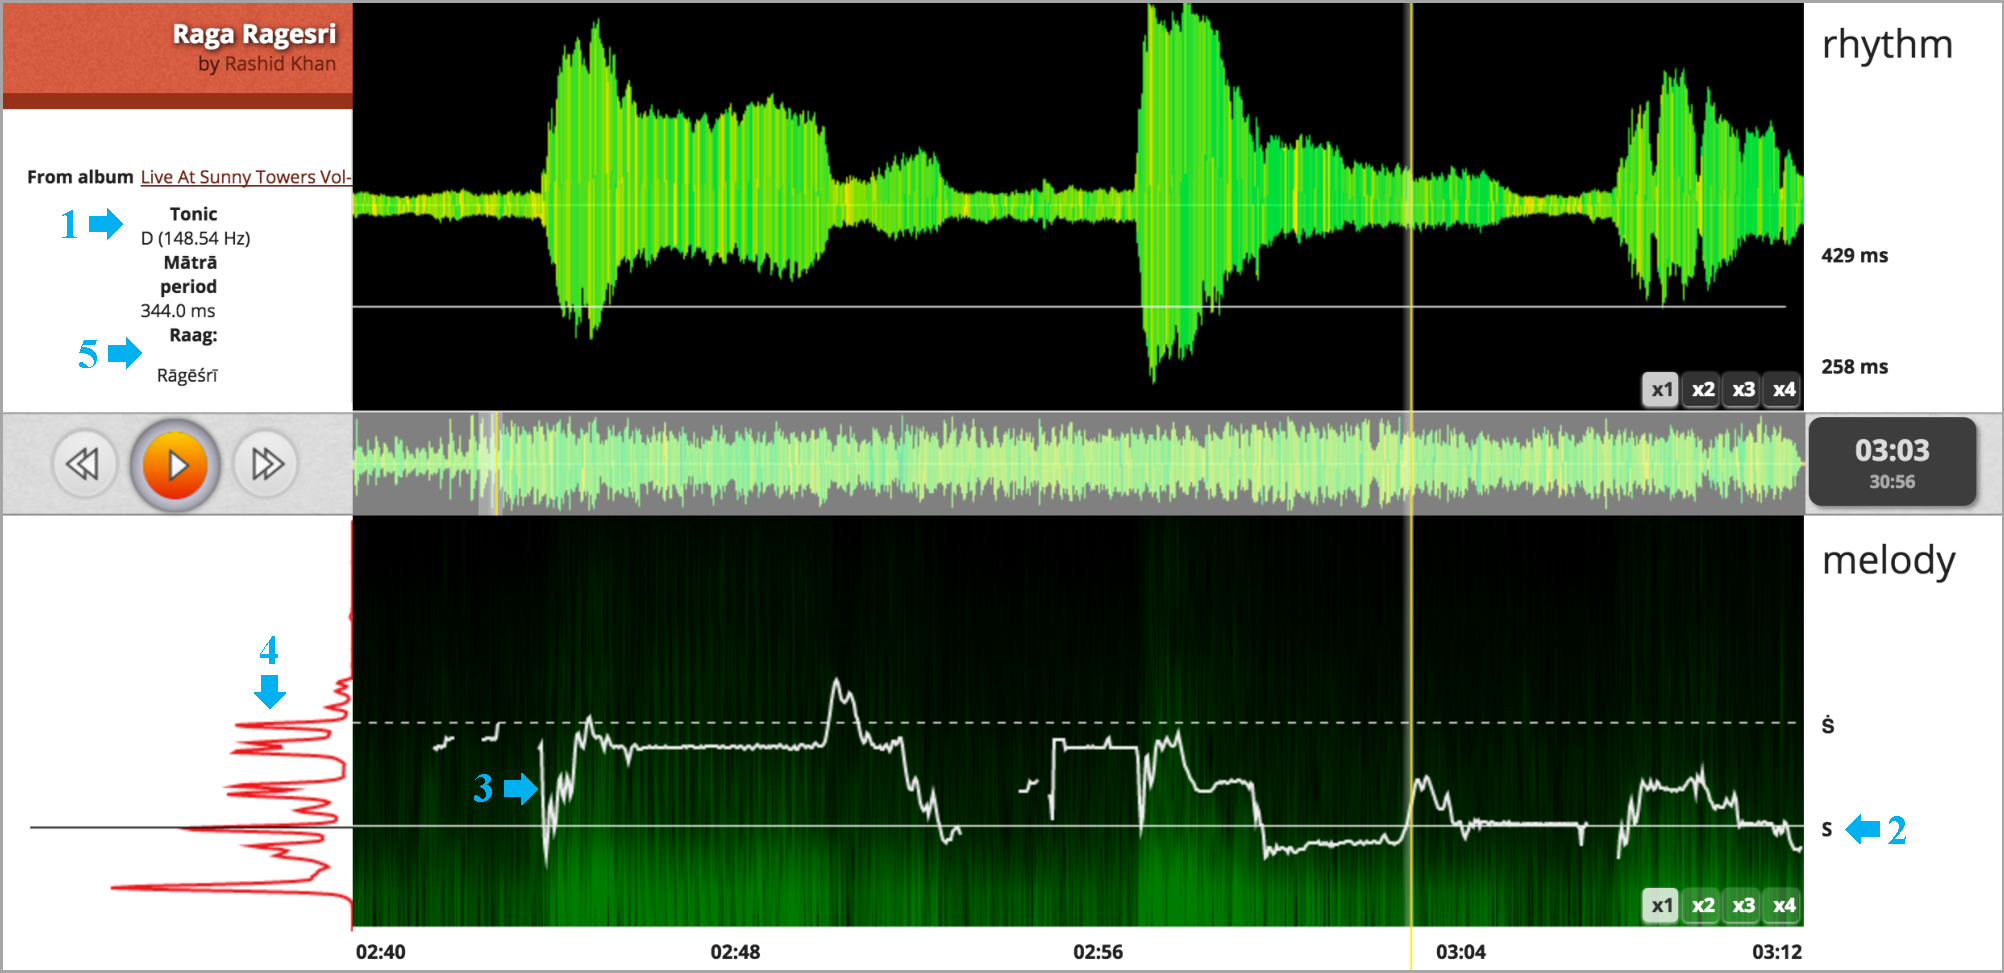
\includegraphics[width=\figSizeHundred]{ch08_applications/figures/dunyaScreenshot.pdf}
		\end{center}
		\caption{Screenshot of a recording page in Dunya showing showing extracted audio descriptors and associated metadata. Tonic, pitch histogram and melody is marked by XXX.}
		\label{fig:dunya_recording}
\end{sidewaysfigure}

While the Web interface provides an easy and a quick access to the data, for a more comprehensive access mainly meant for researchers and developers Dunya provides a restful \gls{api}. Through the \gls{api} it exposes audio recordings, gathered metadata and extracted audio descriptors. For researchers who wish to create datasets from the CompMusic music corpora, such a tool can be very helpful. To further facilitate the usage of Dunya \gls{api}, a Python\footnote{\url{https://www.python.org/}} wrapper, \gls{pycompmusic}\footnote{\url{https://github.com/MTG/pycompmusic}}, is provided. Using this tool with just a few lines of code the entire corpora and associated metadata can be retrieved. An example of an \gls{api} call through \gls{pycompmusic} and the returned Json object corresponding to this call is shown in~\figref{fig:api_call_example}.  

\begin{figure}
	\begin{center}
		
\includegraphics[width=\figSizeHundred]{ch08_applications/figures/figure_todo.pdf}
	\end{center}
	\caption{An example of a code that uses \gls{pycompmusic} Python package to access Dunya data.}
	\label{fig:api_call_example}
\end{figure}

\TODO{Think more, what is left?}


\section{Mobile Applications: Sar\={a}ga and Riy\={a}z}
\label{sec:mobile_apps_camut}

\gls{camut} is a project that aims to explore the commercial exploitation of the technologies developed in the CompMusic project. \gls{saraga} and \gls{riyaz} are the two mobile applications developed as a part of this project that aim to foster learning, teaching and appreciation of Indian music forms. Both these applications incorporate parts of the outcome of our research work presented in this thesis. We provide below a brief description of these applications. 

\subsubsection{Sar\={a}ga}
\label{sec:saraga}

\begin{figure}
	\centering
	\begin{subfigure}[b]{0.48\textwidth}
		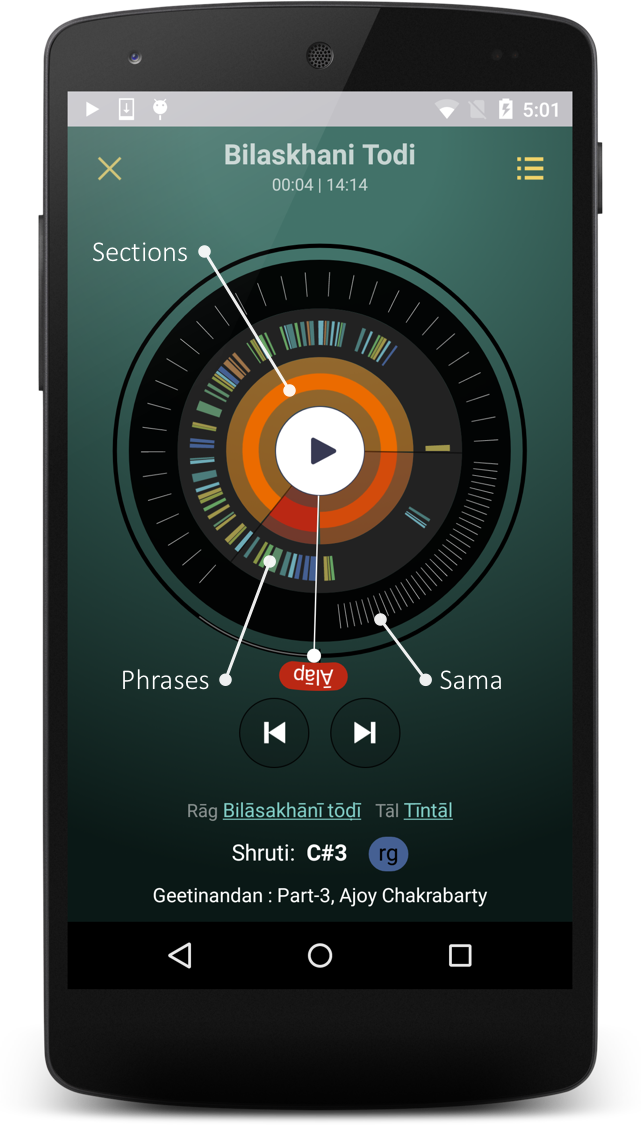
\includegraphics[width=\textwidth]{ch08_applications/figures/saraga1.png}
		\caption{Full music piece}
		\label{fig:saraga_full_piece}
	\end{subfigure}
	\begin{subfigure}[b]{0.48\textwidth}
		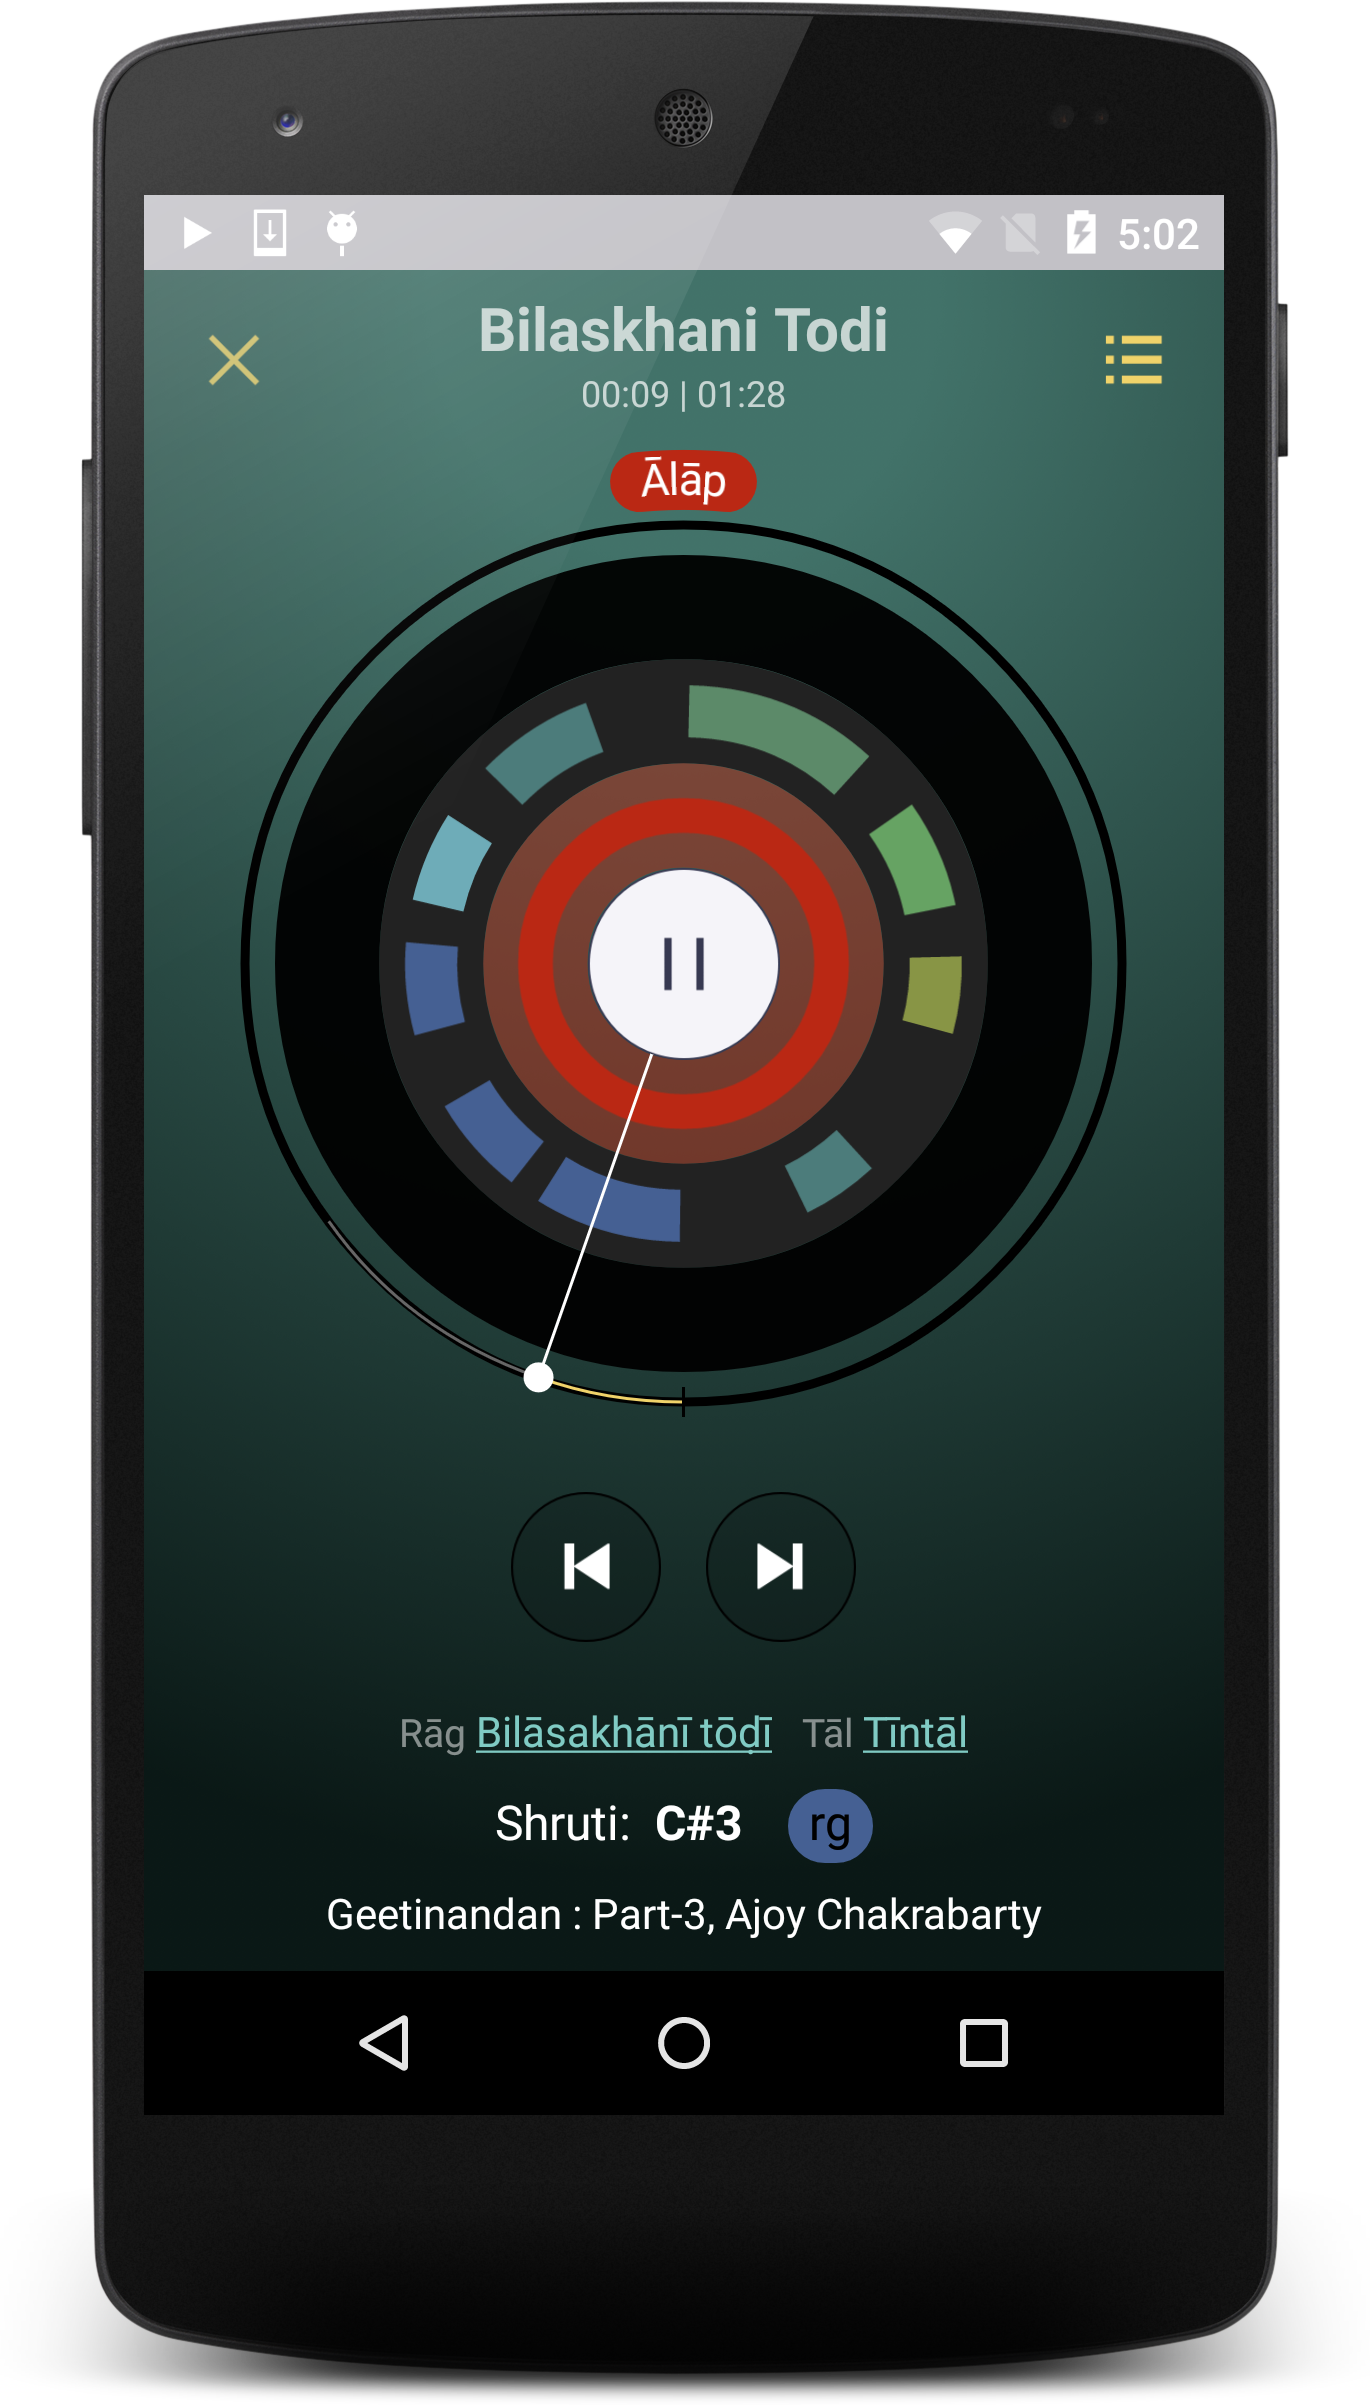
\includegraphics[width=\textwidth]{ch08_applications/figures/saraga2.png}
		\caption{\Gls{alap} section (zoomed in)}
		\label{fig:saraga_alap_section}
	\end{subfigure}
	\caption{Screenshots of Sar\={a}ga mobile application showing a music piece of Hindustani music. (a) shows the entire music piece, (b) shows the \gls{alap} section in the piece. The melodic phrases are marked by colored arches. Tonic (\gls{shruti}) of the recording is shown at the bottom along with the current playing melodic phrase.}
	\label{fig:saraga_screens}
\end{figure}

\Gls{saraga} is a mobile application that provides an enriched listening atmosphere over a collection of Carnatic and Hindustani music that is released under Creative Commons license\footnote{\url{https://creativecommons.org/}}. It is meant for music connoisseurs and students of these art music traditions to navigate, discover and listen the music using culturally relevant concepts. \gls{saraga} includes inclusive designing of innovative visualizations and inter and intra-song navigation interfaces that present musically rich information to the user in a compact way. The time synchronized visualizations of musically relevant facets such as melodic patterns, \gls{sama} locations and sections provides a user with better understanding and appreciation of these music traditions.

In~\figref{fig:saraga_screens} we show a screenshot of the recording page of in \gls{saraga} playing a music piece\footnote{\url{https://musicbrainz.org/recording/3124479b-5118-4cf3-823f-8fefad45e586}} in Hindustani music. In~\figref{fig:saraga_screens}\,(a) the entire music piece is visualized. Information regarding the sections, melodic patterns and the \gls{sama} locations is shown contained in the concentric circles as indicated in the screenshot. As the playback advances in time along the circle, these descriptors are highlighted based on the current time. For example, in~\figref{fig:saraga_screens}\,(a) the melodic phrase ``rg'' is being sung in the piece, which is highlighted at the bottom of the screen. Since the music performances in \gls{iam} can last long (sometimes up to an hour), \gls{saraga} interface allows to tap and zoom into a particular section. An example of this is shown in~\figref{fig:saraga_screens}\,(b) wherein the \gls{alap} section is selected. Furthermore, a user can also tap on a particular melodic pattern to then go to a new page where all the occurrences of that pattern in the recording are shown together. These functionalities facilitate a user to better understand the structuring of different musical facets in a piece of \gls{iam}. In addition to these descriptors there is accompanying data shown at the top and the bottom of the screen, which includes editorial metadata and \gls{shruti} (tonic) information. The text strings corresponding to the musical concepts (\gls{raga} and \gls{tala}) are hyper-linked to their respective pages, where that musical concept is described through a bunch of representative audio examples. 


\subsubsection{Riy\={a}z}
\label{sec:riyaz}




\gls{riyaz} is a mobile application that aims to facilitate music learning for beginner to intermediate level music students of \gls{iam} by making their practice sessions more efficient. It does it by simulating a classroom environment in which the learning happens through imitating the musical exercises build by processional musicians. The application performs singing assessment and provides a detailed feedback, wherein it highlights the mistakes and gives suggestions to improve. In~\figref{fig:riyaz_evaluation_screen} we show the main evaluation screen of \gls{riyaz} where a user can visualize in real-time the pitch track and \gls{svara} score. Post practice session a detailed feedback is provided as shown in~\figref{fig:riyaz_feedback_screen}.  Note that \gls{riyaz} is a work in progress with a prototype version already available at the time of writing this thesis. Currently there are 1000+ users with 15000+ user sessions. 

\begin{figure}[h]
	\begin{center}
		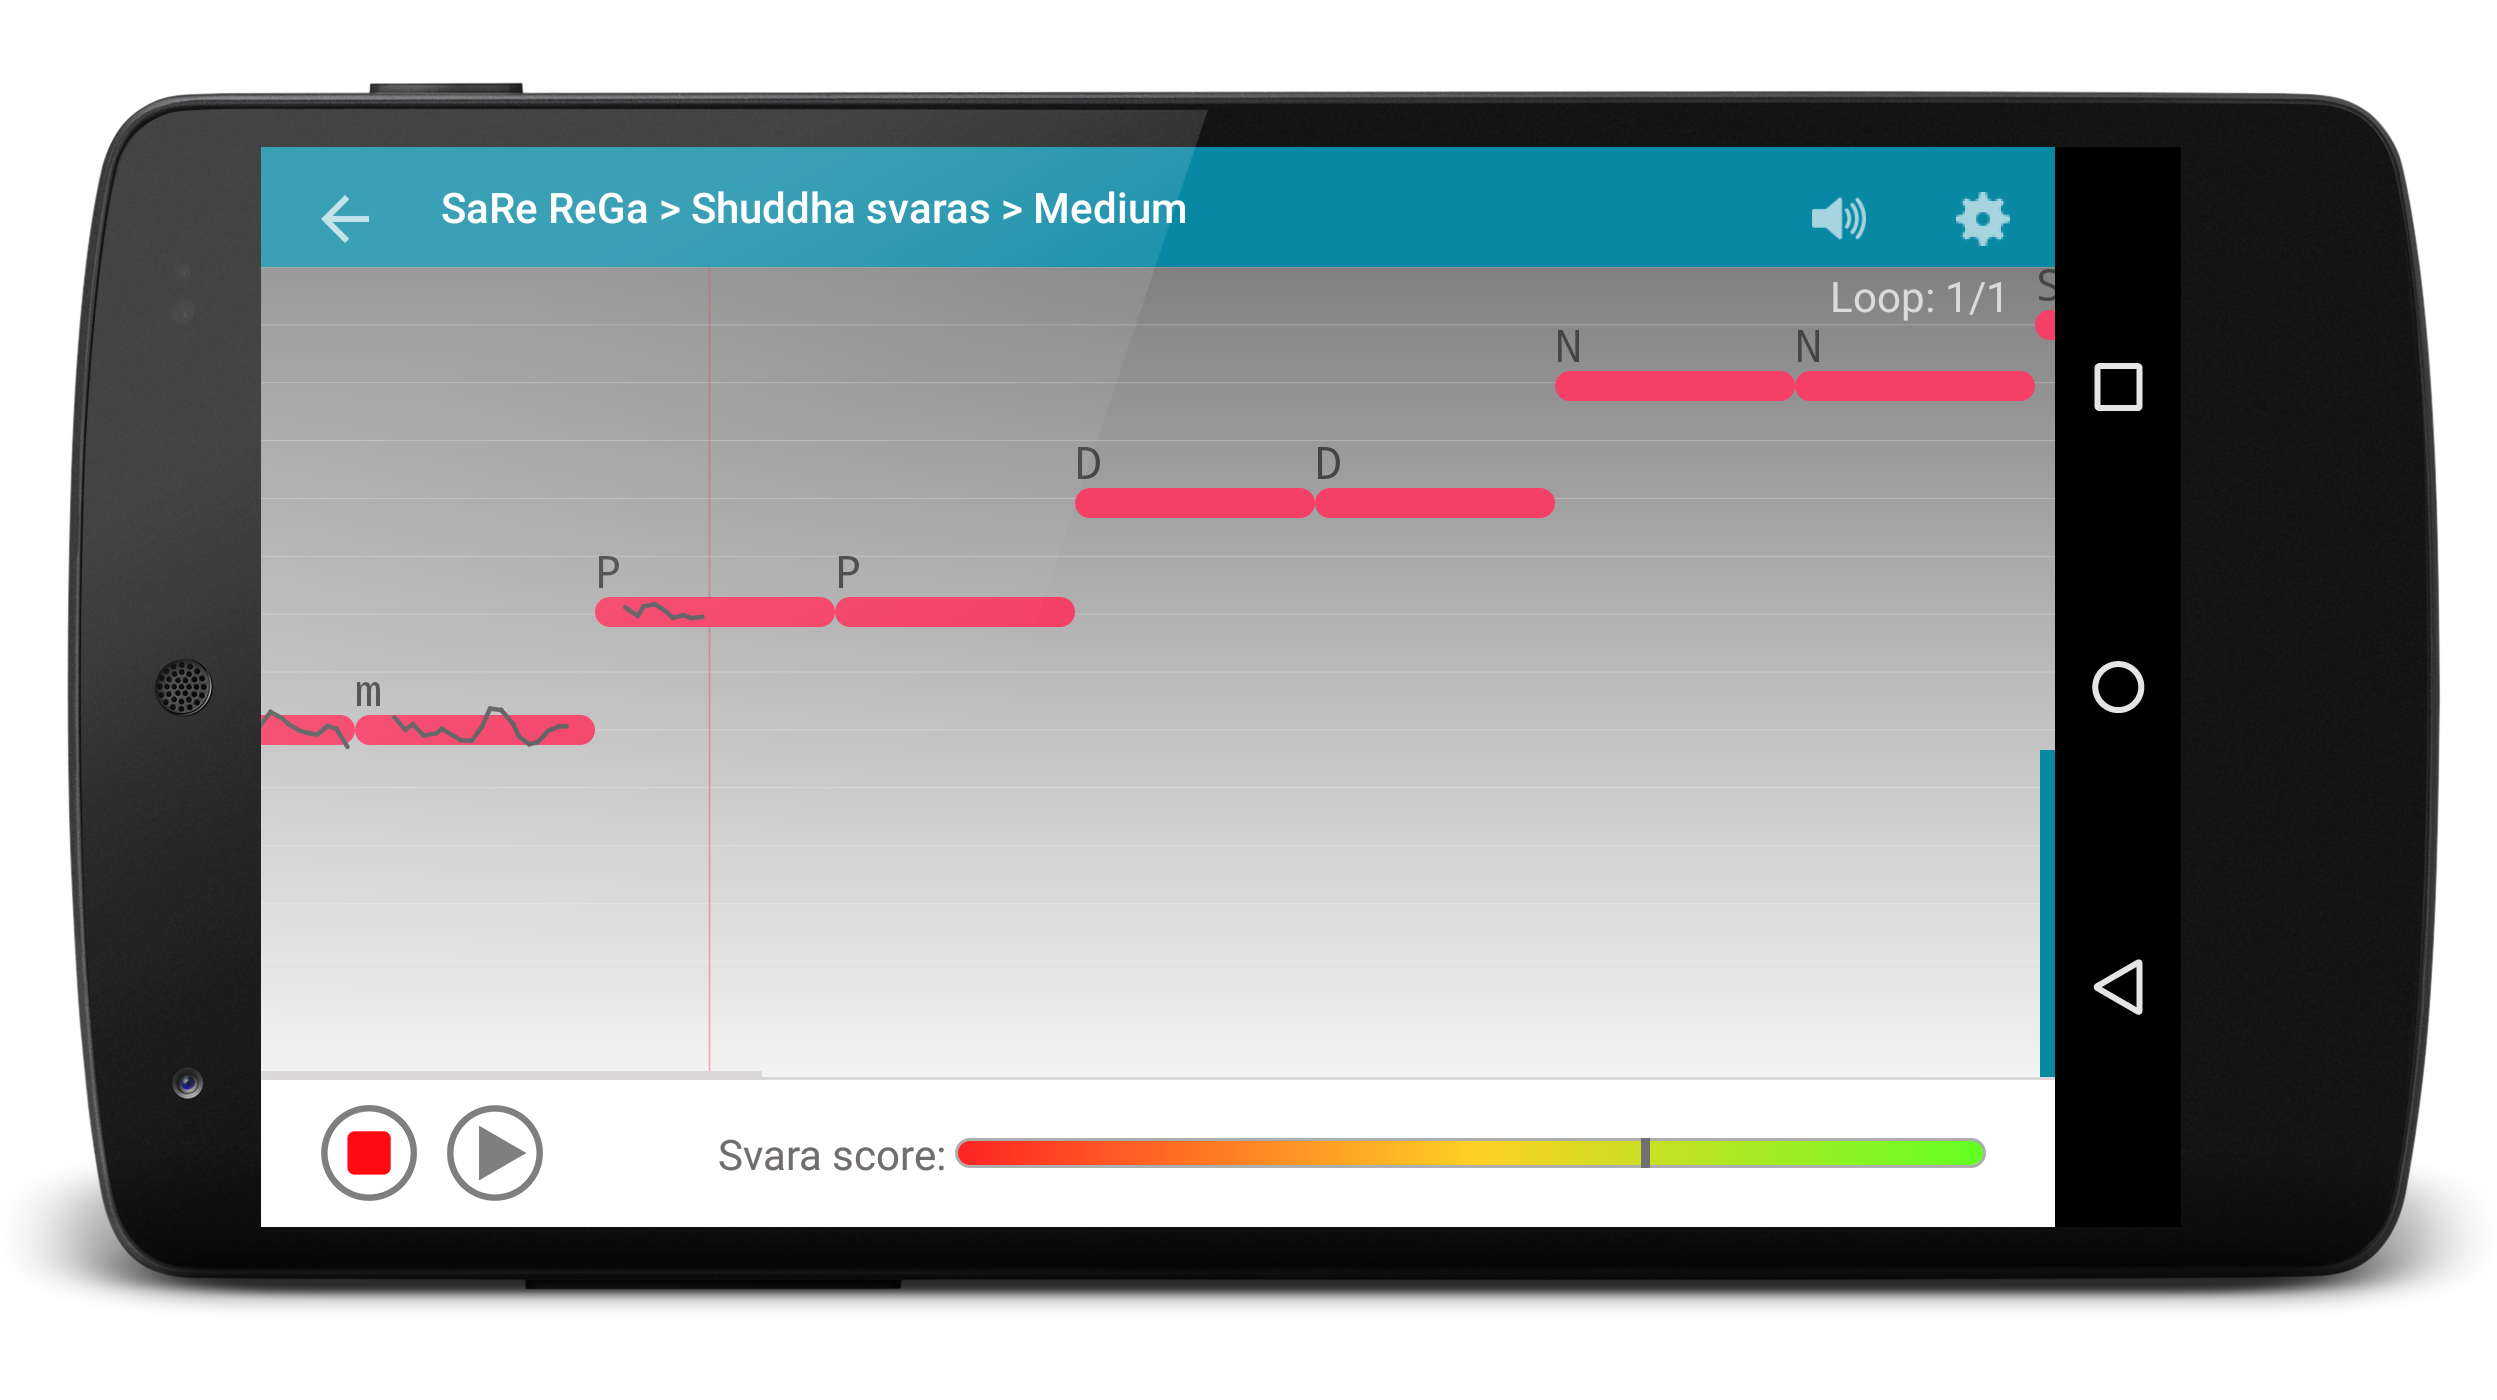
\includegraphics[width=\figSizeEighty]{ch08_applications/figures/riyaz1.png}
	\end{center}
	\caption{Screenshot of the evaluation screen in Riy\={a}z (Beta) mobile application showing real time melody extraction and scoring.}
	\label{fig:riyaz_evaluation_screen}
\end{figure}
\begin{figure}[h]
	\begin{center}
		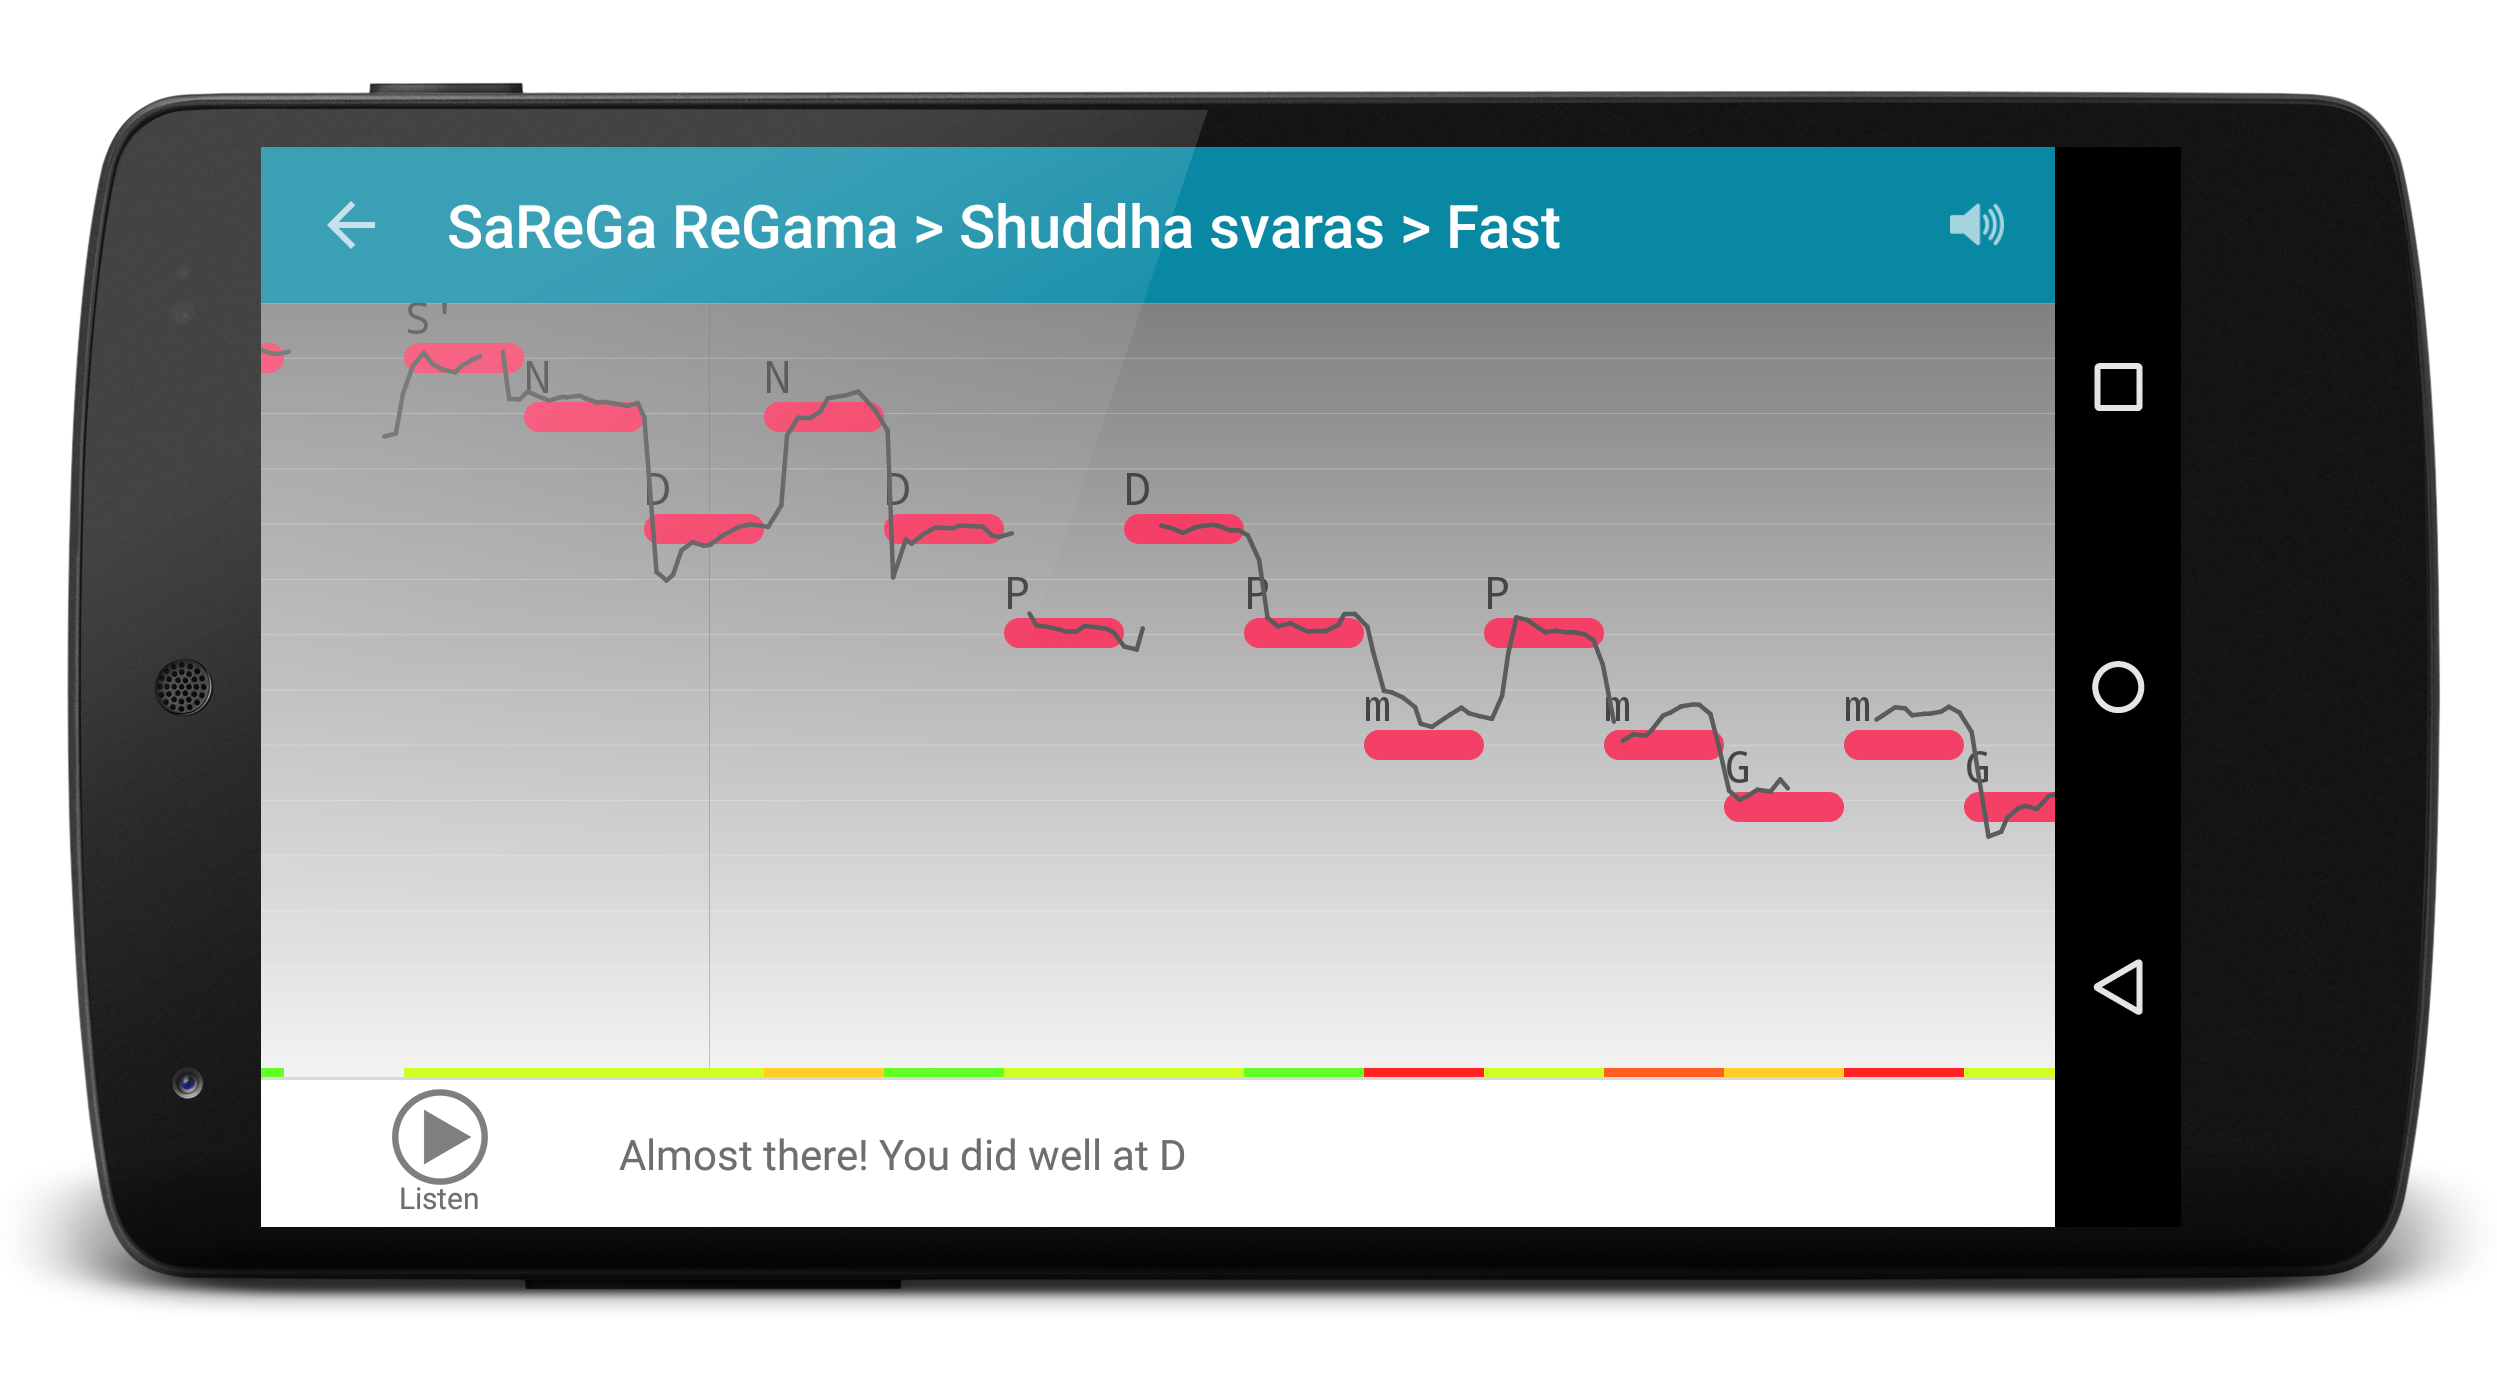
\includegraphics[width=\figSizeEighty]{ch08_applications/figures/riyaz2.png}
	\end{center}
	\caption{Screenshot of the feedback screen in Riy\={a}z (Beta) mobile application showing detailed feedback}
	\label{fig:riyaz_feedback_screen}
\end{figure}



\section{Demos}


\subsection*{Demo1: Melodic Phrase-based Navigation of Collection}


\begin{figure}
	\begin{center}
		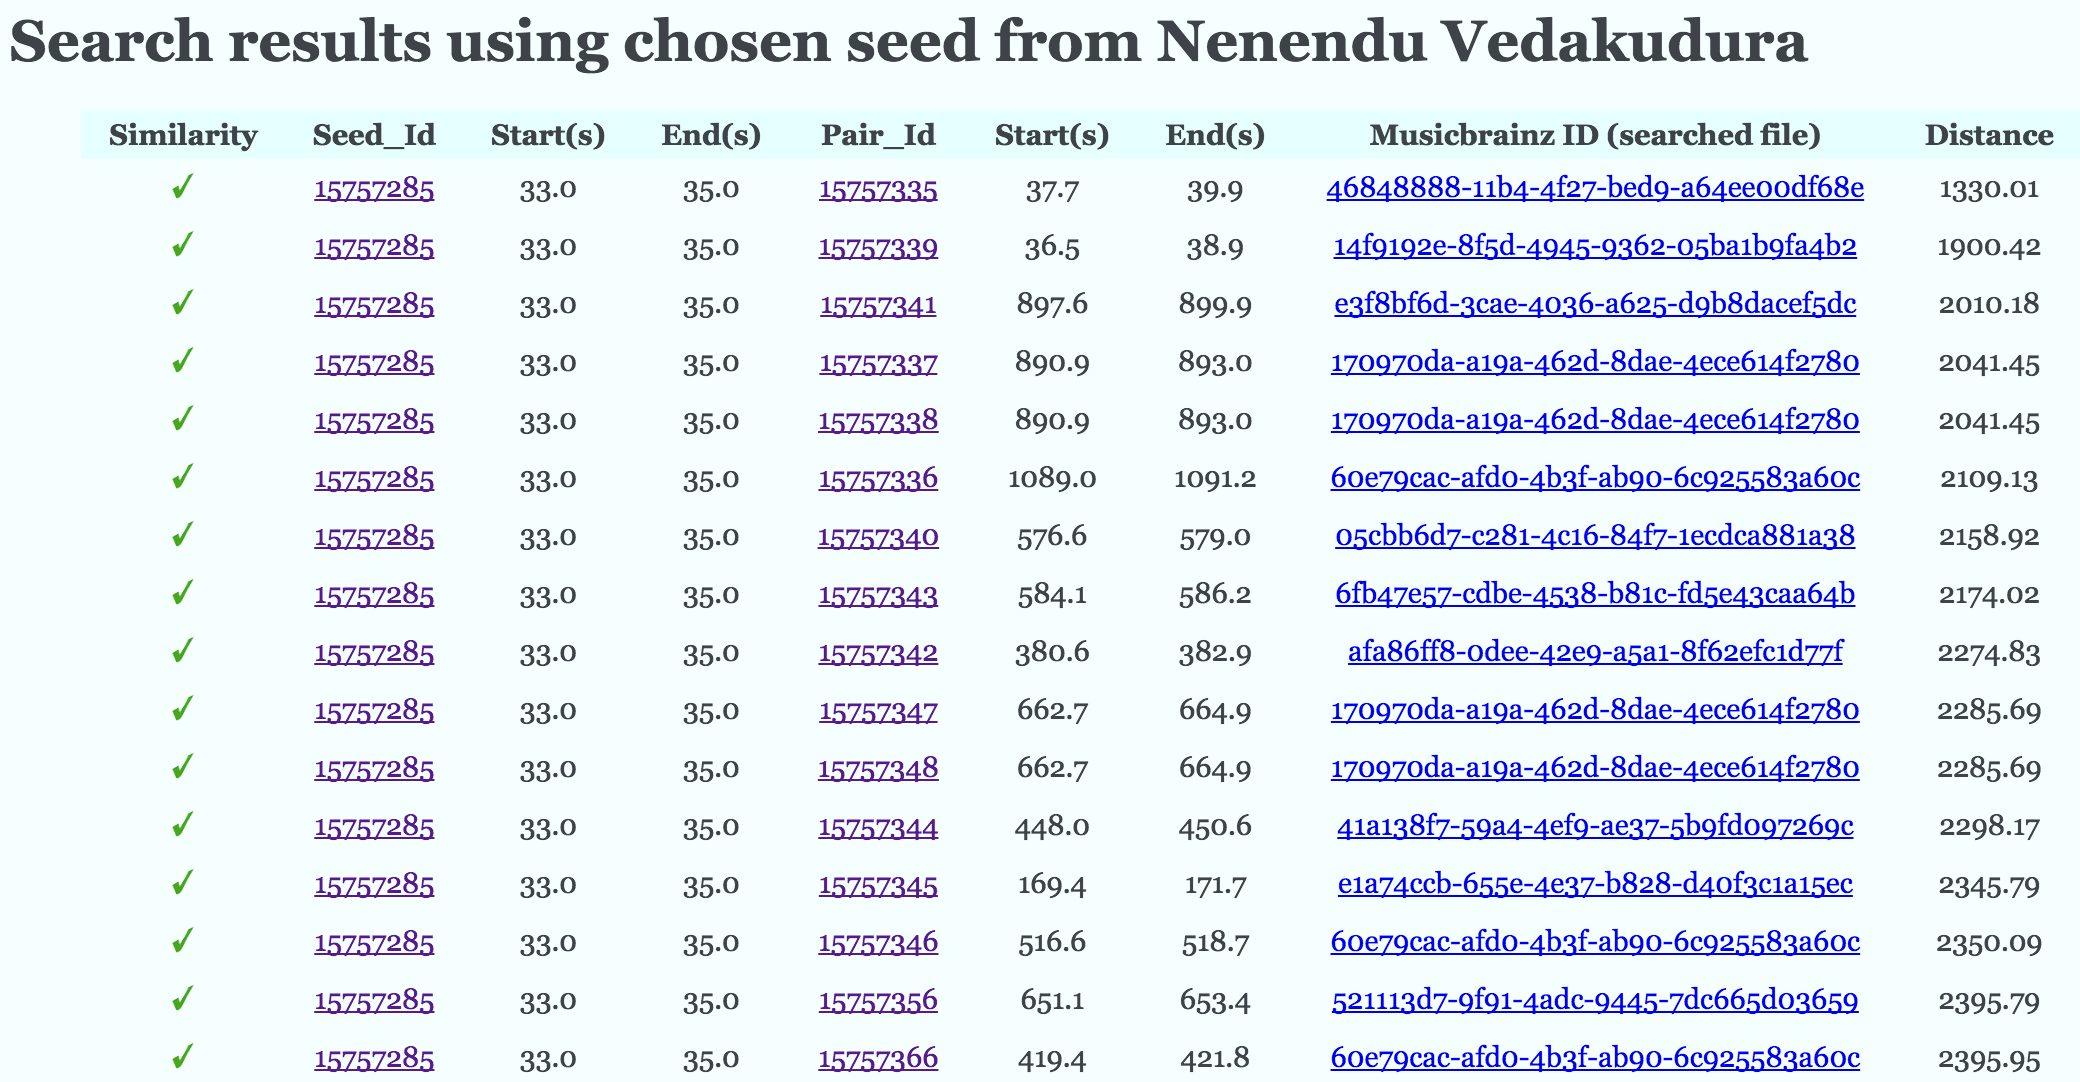
\includegraphics[width=\figSizeHundred]{ch08_applications/figures/patternBrowsing1.png}
	\end{center}
	\caption{Screenshot of a Web demo for navigating through the discovered melodic patterns organized by artists, releases and recordings.}
	\label{fig:browser_patterns}
\end{figure}

\subsection*{Demo2: Melodic Phrase-based Similarity Spaces}

\begin{figure}
	\begin{center}
		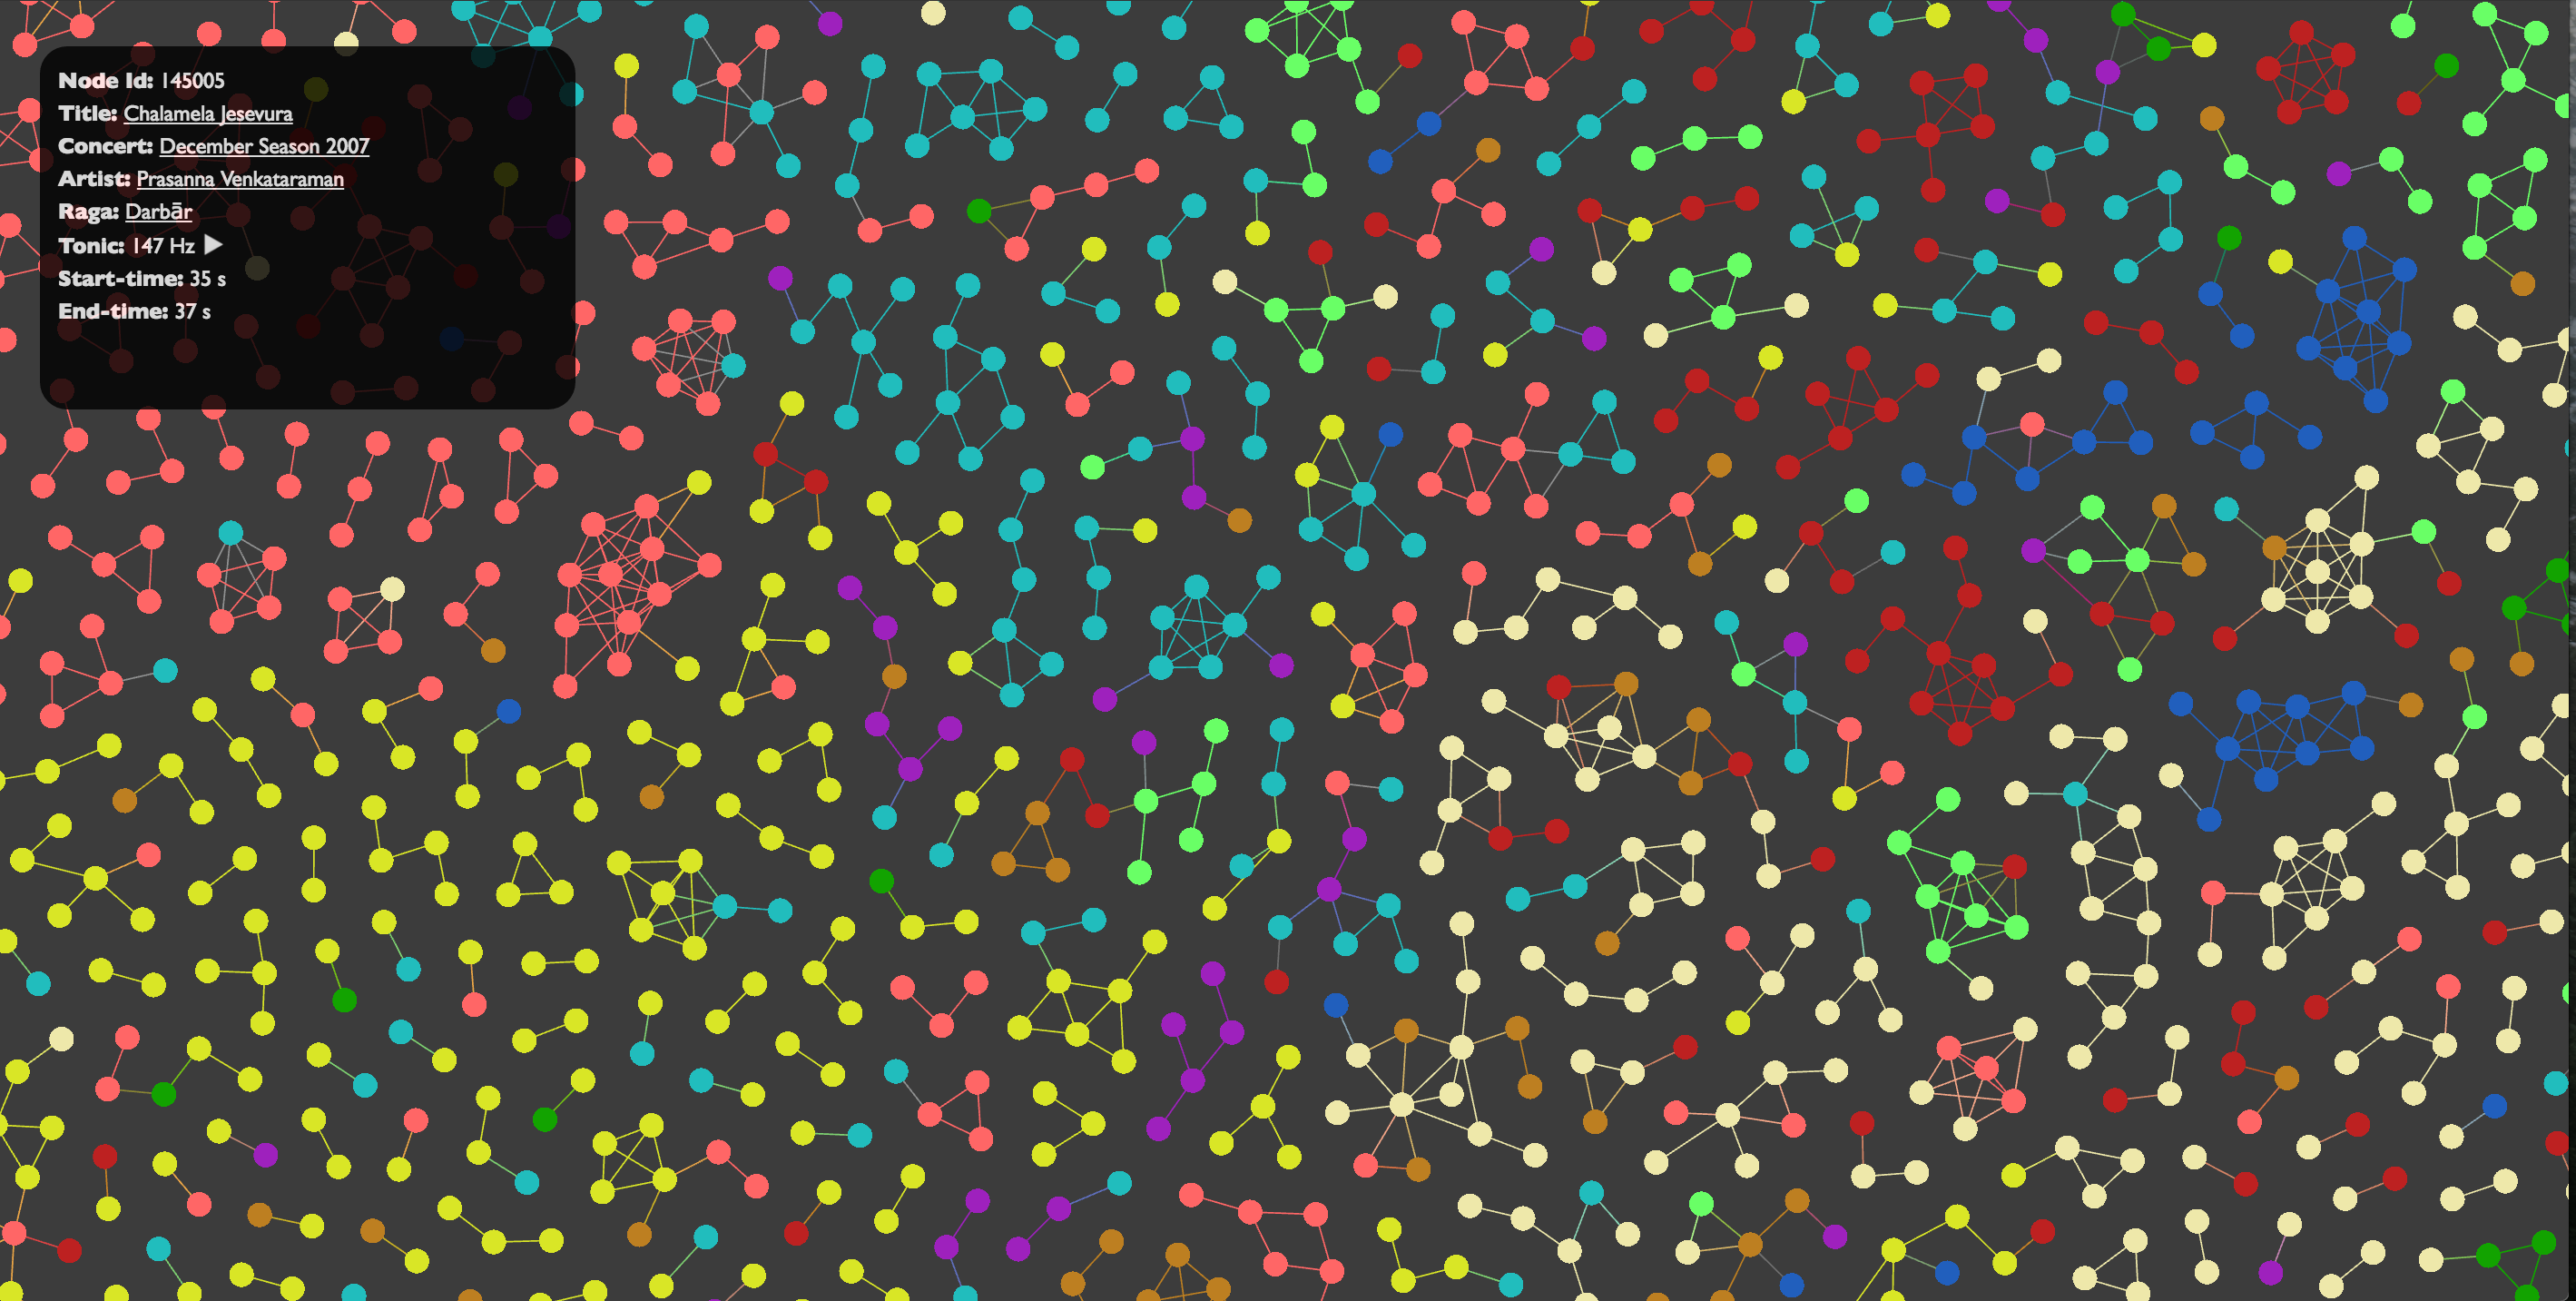
\includegraphics[width=\figSizeHundred]{ch08_applications/figures/patternNetwork1.png}
	\end{center}
	\caption{Screenshot of a Web demo of a network of the discovered melodic patterns. Colors indicate different \glspl{raga}.}
	\label{fig:network_patterns}
\end{figure}



\subsection{Ragawise: Realtime Raga Recognition}
\label{sec:ragawise}

\begin{sidewaysfigure}
	\begin{center}
		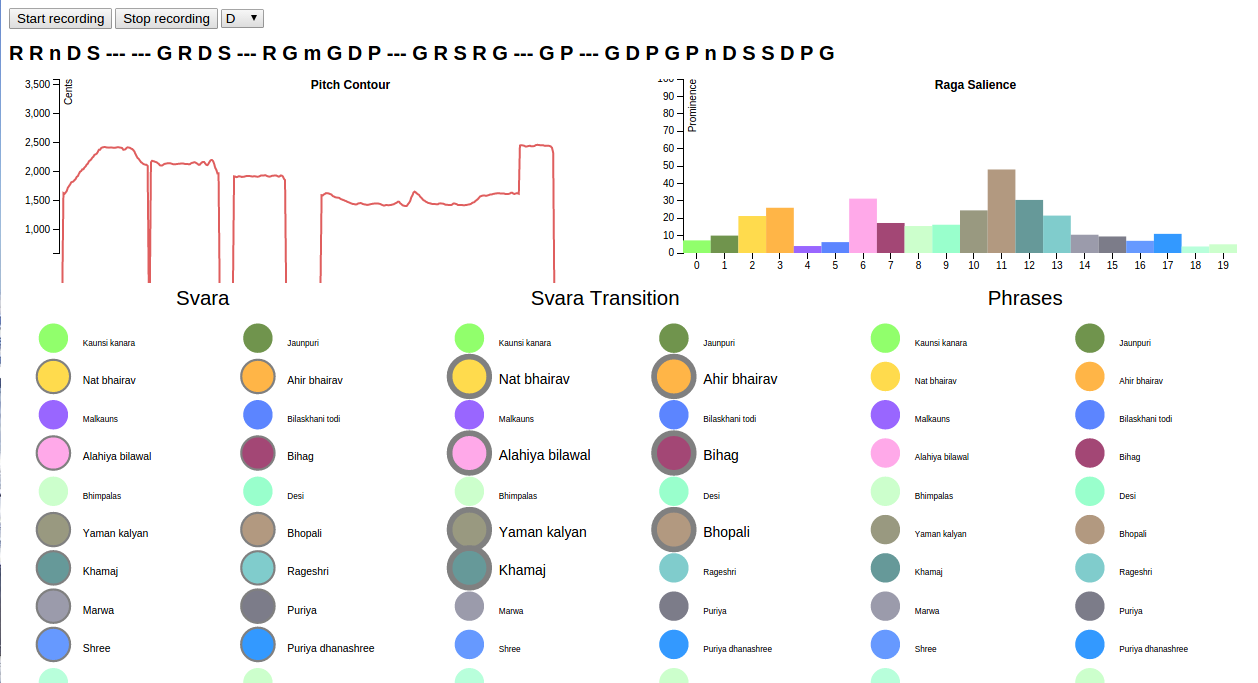
\includegraphics[width=\figSizeHundred]{ch08_applications/figures/ragawise.png}
	\end{center}
	\caption{Screenshot of Ragawisea recording page in Dunya showing showing extracted audio descriptors and relevant editorial metadata. Tonic, pitch histogram and melody is marked by XXX.}
	\label{fig:dunya_recording}
\end{sidewaysfigure}


\section{Tools for Musicological Studies}
\COMMENT{Write this section if you get time at the end}

\section{Summary}



